\section{AES}
\textit{Advance Encryption Standard}, or AES, is a non-Feistel cipher.
\subsection{General info}
\begin{itemize}
    \item Block size: 128 bits
    \item Key size: 128/192/256 bits
    \item Rounds: 10/12/14
\end{itemize}
\subsection{Number Theory}
{\color{blue} [skip modular addition, multiplication,etc.]}

\subsection{Galois Fields}
For a given prime $p$, we can define the \textit{finite field of order $p$}, $GF(p)$, as the set $Z_p$ of integers ${0,...,p-1}$ together with the arithmetic operations $\Mod p$.
In order to not waste bit and "fit" directly a finite field into our bytes, we need $GF(2^n)$, but they works differently when using operations.
\subsubsection{Polynomial Arithmetic}

$GF(p^n)$ means that 
\begin{itemize}
    \item we want coefficients in $GF(p)$ ($p=2\rightarrow$ coefficients can only be 0 or 1)
    \item the result of each operations as to be reduced using $\Mod{m(x)}$ where $m(x)$ is some irreducible polynomial with order $n$
\end{itemize}
\begin{center}
    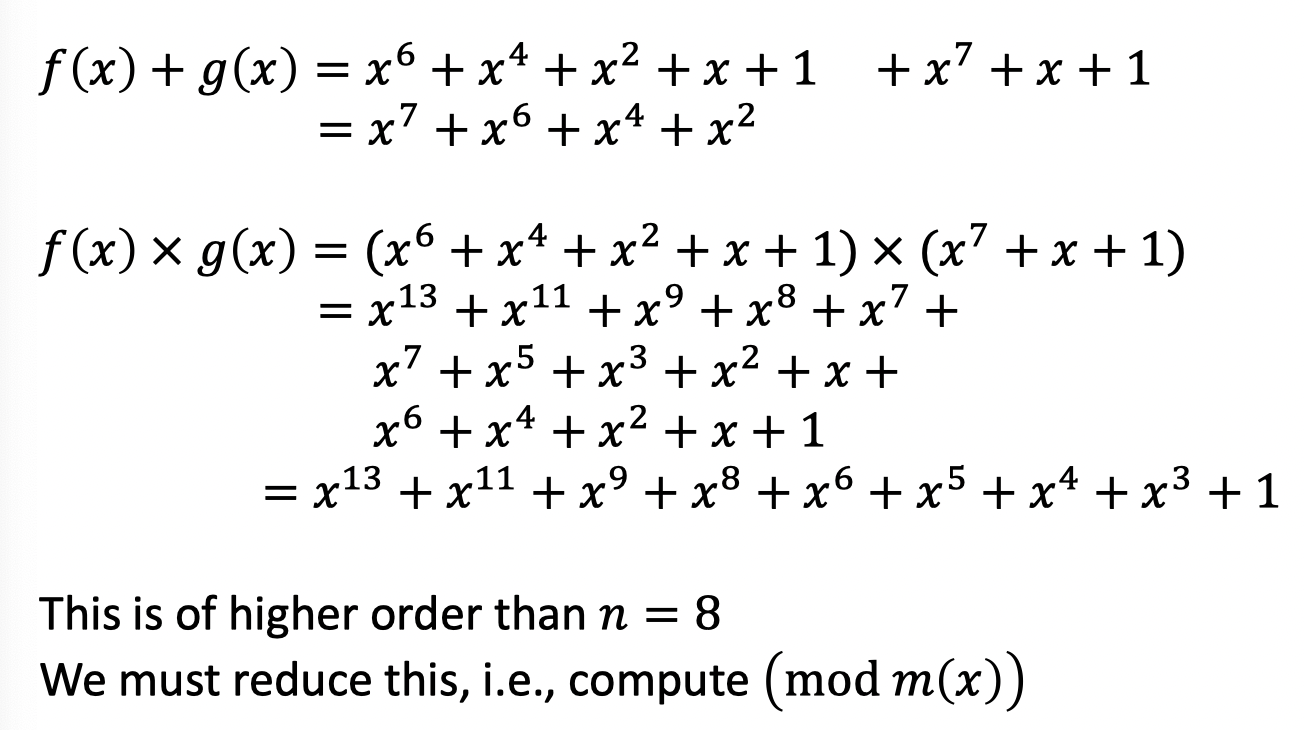
\includegraphics[scale=0.2]{images/gf1.png}
    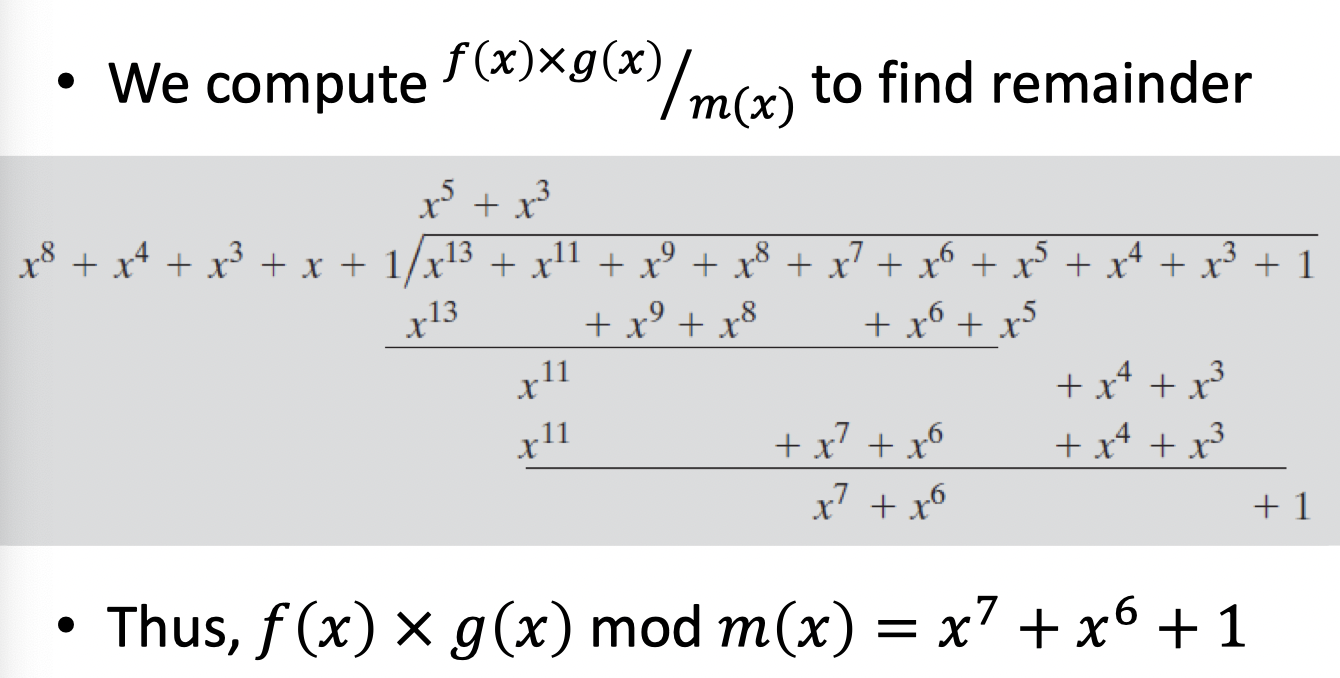
\includegraphics[scale=0.2]{images/gf2.png}
\end{center}

\subsection{AES Structure}
\begin{enumerate}
    \item \textbf{Substitute bytes}: uses an S-box to perform a $b$ byte substitution of the block
    \item \textbf{ShiftRows}: A simple permutation
    \item \textbf{MixColumns}: A substitution that makes use of arithmetic over GF($2^8$)
    \item \textbf{AddRoundKey}: A simple bitwise XOR of the current block with a portion of the expanded key
\end{enumerate}
AES begins with AddRoundKey, followed by $9$ rounds (128-bit) with all $4$ stages and final round with only $3$ stages (skip MixColumns). In order to have the right length for the key, we also perform a \textbf{key expansion}.